\documentclass{article}
\usepackage [T2A] {fontenc}
\usepackage[utf8]{inputenc}
\usepackage[russian,english]{babel}
\usepackage{amsmath,amssymb}
\usepackage[pdftex]{graphicx}
\begin{document}
А. Т. Улимаева
\\(г. Уфа)
\\РЕШЕНИЕ ЗАДАЧ НА НАХОЖДЕНИЕ НАИБОЛЬШИХ И НАИМЕНЬШИХ ЗНАЧЕНИЙ ФУНКЦИЙ
\\Опыт нашей работы в школах Башкирской АССР показал, что при организации повторения учебного материла в Х классе целесообразно рассматривать задачи на нахождение наибольших и наименьших значений функций, причем использовать при их решении наряду с аппаратом производной и другие способы. Это способствуют активизации мыслительной деятельности учащихся, вызывает у них интерес к решению задач и к изучению математики в целом.
\\Приведем пример решения одной такой задачи:
\\Требуется оградить прямоугольный участок земли площадью $a^2$. Определите оптимальные размеры участка, при которых затраты на ограду будут наименьшими (предполагается, что стоимость ограды пропорционально ее длине с коэффициентом $k>0$).
\\Решение. I способ. Найдем прямоугольник площади $a^2$, у которого периметр наименьший. Пусть $x>0$ -- длина стороны прямоугольника, тогда длина смежной с ней стороны равна $\frac{a^2}{x}$. Периметр прямоугольника $P(x)=2(x+\frac{a^2}{x})$.
\\Найдем наименьшее значение $P(x)$, применяя производную:
$$P'(x)=2(1-\frac{a^2}{x^2}), x\in]0;+\infty[$$
\\Определим критические точки функции:
$$(2(1-\frac{a^2}{x^2})=0)\Leftrightarrow(x=a\mbox{ или }x=-a)$$
\\так как $a>0$, то $x=a\in]0,+\infty[$.
\\Найдем следующие значения функции $P'(x)$:
$$P'(\frac{a}{2})=2(1-\frac{4a^2}{a^2})=-6<0$$
$$P'(2a)=2(1-\frac{a^2}{4a^2})=\frac{3}{2}>0$$
\\Следовательно, $\min\limits_{]0;+\infty[}P(x)=4a$ при $x=a$.
\\Длина другой стороны прямоугольника также равна $a$.
\\Из условия задачи известно, что стоимость изгороди $N(x)$ пропорциональна ее длине с коэффициентом $k>0:N(x)=k\cdot P(x)$. Следовательно $N(x)$ получит наименьшее значение, откуда 
$$N_{opt}(x)=\min\limits_{]0;+\infty[}N(x)=k\cdot4a\mbox{ при }x=a$$
\\Итак, чтобы оптимизировать стоимость изгороди, целесообразно выбрать участок квадратной формы.
\\II способ. Замечая, что $P(x)=2(x+\frac{a^2}{x})=2((\sqrt{x})^2-2\sqrt{x}\frac{a}{\sqrt{x}}+\frac{a^2}{(\sqrt{x})^2})+4a=2(\sqrt{x}-\frac{a}{\sqrt{x}})^2+4a$, где $x\in]0;+\infty[$, заключаем, что $\min\limits_{]0;+\infty[}P(x)=4a$ при $x=a$:
$$((\sqrt{x}-\frac{a}{\sqrt{x}})^2=0)\Rightarrow(\sqrt{x}=\frac{a}{\sqrt{x}})\Rightarrow(x=a)$$
\\III способ. Обозначим полупериметр прямоугольника $p(x)$. Пусть x -- длина одной из его сторон, тогда длина смежной с ней стороны равна $p-x(0\leqslant x\leqslant p)$. Площадь прямоугольника $a^2=x(p-x)$;
$$(x^2+a^2-px=0)\Leftrightarrow((x-a)^2+x(2a-p)=0$$
\\Последнее равенство истинно лишь при $2a-p\leqslant0$, т. е. при $p\geqslant2a$. Следовательно, наименьшее значение полупериметра равно 2a.
\\Подставляя в уравнение $x^2+a^2-px=0$ наименьшее значение $p$, получим уравнение $x^2-2a+a^2=0$, откуда $x=a$.
\\VI способ. Обозначим длины смежных сторон прямоугольника через $x$ и $y$, а его полупериметр через p. Тогда $xy=a^2$.
\\Чтобы найти наименьшее значение периметра прямоугольника площади $a^2$, воспользуемся известным тождеством: $(x+y)^2=(x-y)^2+4xy$. Заменив в нем произведение $xy$ на равное ему значение $a^2$, получим равенство
$$(x+y)^2=(x-y)^2+4a^2$$
\\Из этого равенства видно, что выражение $(x+y)^2=p^2$ получит наименьшее значение при $x-y=0$, т. е. при $x=y$. Полупериметр $p=x+y$ достигает своего наименьшего значения при $x=y=a$, при этом $P=4a$. 
\\V способ. По условию $xy=a^2$, где $x$ и $y$ -- длины смежных сторон прямоугольника.
\\Предположим, что $x\neq y$, пусть, например, $x=a+b(b>0)$, тогда 
$$y=\frac{a^2}{a+b}>\frac{a^2-b^2}{a+b}=a-b$$
\\Значит, $x+y>a+b+a-b=2a$.
\\Пусть теперь $x=y=a$. В этом случае $x+y=2a$.
\\Имеем: $x+y\geqslant2a$, откуда следует, что наименьшее значение периметра прямоугольника равно $4a$ и достигается оно при $x=y=a$
\\VI способ. К решению задачи можно применить также геометрические построения. В условии задачи дано: $xy=a^2$, где $x$ и $y$ -- длины смежных сторон прямоугольника.
\\При $x=y=a(a>0)$ получаем $x+y=2a$. Построим окружность с центром в точке $O$ радиуса $|AO|=a$. Имеем: $|AB|=|AO|+|OB|=x+y=2a$ (см. рис.).
\\
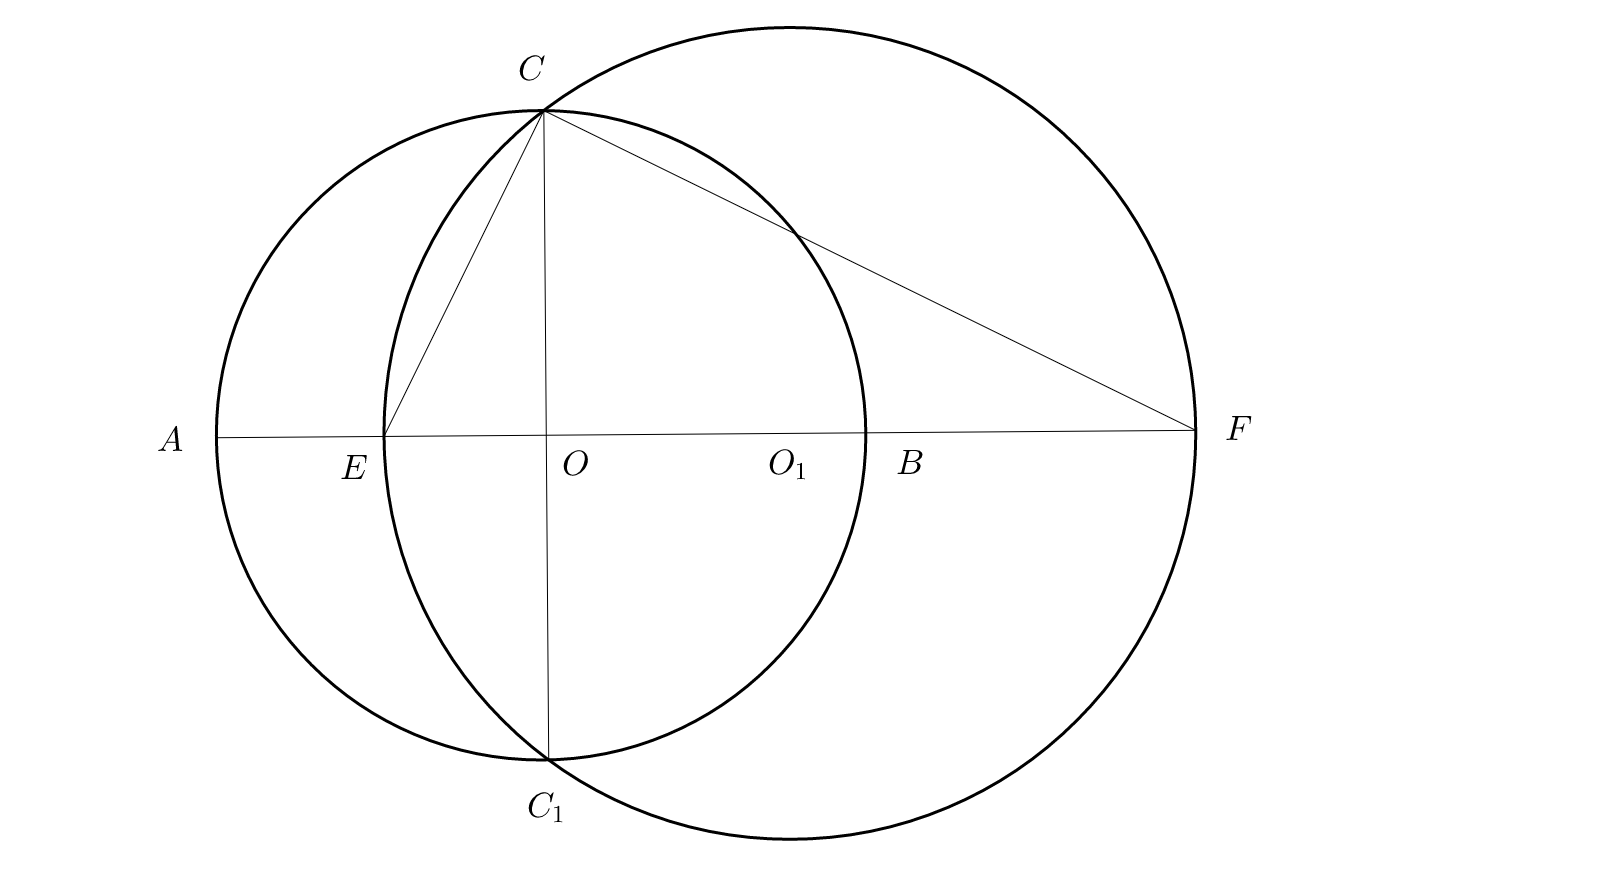
\includegraphics[scale=0.25]{circle.png}
\\Пусть $x\neq y$. Построим на том же рисунке окружность с центром в точке $O_1$ и радиусом, равным длине отрезка $O_1F$, так, чтобы $|EO|\cdot|OF|=a^2$. Тогда $|EO|+|OF|=|EF|$, где $|EO|=x$, $|OF|=y$.
\\Рассматривая рисунок, замечаем, что $|EF|>2a$, так как $|EF|$ -- длина диаметра, а $2a$ -- длина хорды $CC_1$ окружности $(O_1,|O_1F|)$. Таким образом получаем, что $x+y\geqslant2a$, причем $x+y=2a$ при $x=y=a$.
\end{document}